
\documentclass{article}
\usepackage{amsmath}
\usepackage{listings}
\usepackage{graphicx}
\usepackage[margin=1in]{geometry}
\pagenumbering{gobble}
\setlength{\tabcolsep}{10pt}
\renewcommand{\arraystretch}{1.7}
 
\begin{document}

\section*{\hfil A. Mengurutkan Bilangan\hfil}

\subsection*{Deskripsi}

\par\noindent Arka, seorang perancang puzzle terkenal, sedang merancang puzzle baru yang ia namakan Snake Cube. Berikut adalah detail tentang puzzle yang ia buat:

\begin{itemize}
	\item Terdapat 27 kubus kecil yang memiliki ukuran yang sama.
	\item Kubus-kubus kecil tersebut akan dirangkai sedemikian sehingga setiap kubus kecil akan menempel dengan dua kubus kecil lain, kecuali dua kubus kecil yang hanya menempel dengan satu kubus kecil lain. Kedua kubus kecil tersebut disebut sebagai ujung rangkaian.
	\item Setiap kubus kecil dapat diputar terhadap kubus kecil yang menempel dengan kubus tersebut. Untuk lebih jelasnya, silakan lihat contoh putaran di bawah ini.

	\begin{figure}[h!]
		\centering
		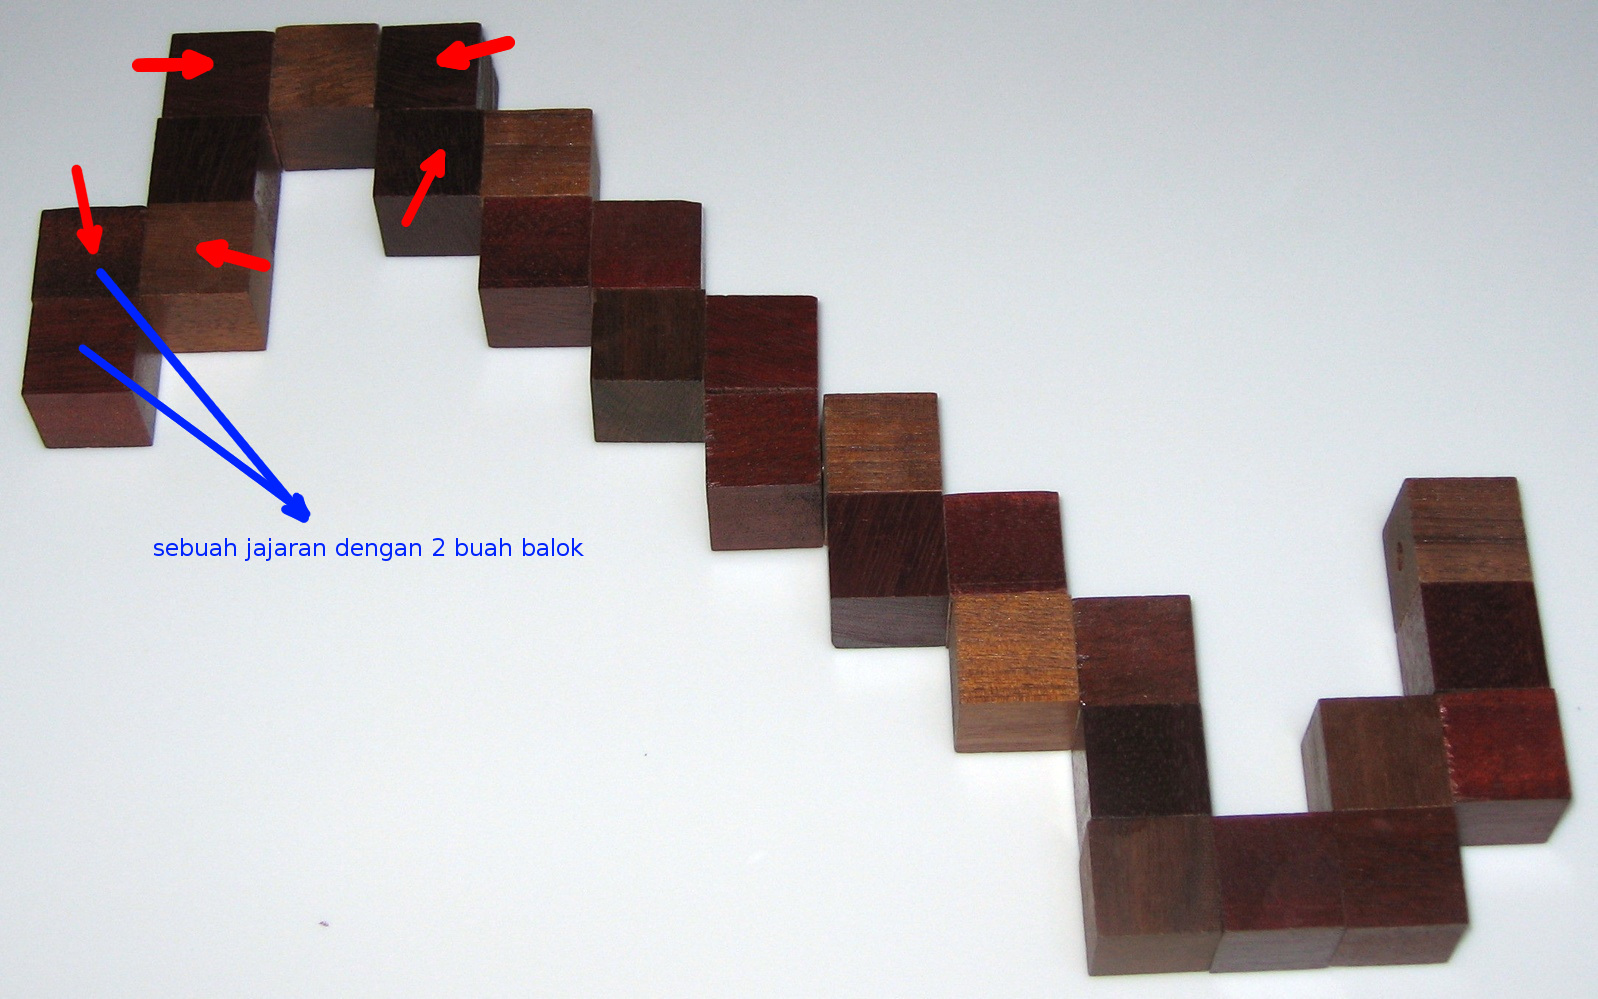
\includegraphics[width=0.5\linewidth]{contoh-1.jpg}
		\caption{https://www.jedicreations.com/wholesale-games-puzzles/snake-cube.php}
	\end{figure}

	\item Tidak boleh ada lebih dari tiga kubus dalam satu jajaran. Jajaran didefinisikan sebagai subrangkaian yang diawali dan diakhiri oleh ujung jajaran. Ujung jajaran dapat berupa ujung rangkaian atau sendi. Sendi didefinisikan sebagai kubus kecil yang menempel kepada dua kubus kecil lain dan bersama dua kubus kecil tersebut membentuk sudut 90 derajat. Pada gambar di atas, sendi adalah kubus yang ditunjuk oleh panah berwarna merah sedangkan jajaran adalah yang berwarna biru.

\end{itemize}

\par\noindent Adapun tujuan dari puzzle ini adalah merangkai rangkaian kubus-kubus kecil tersebut menjadi sebuah kubus besar berukuran 3x3x3.

\par\noindent Agar puzzle ini terjual banyak, Arka ingin membuat banyak versi rangkaian puzzle yang berbeda. Namun, ada rangkaian-rangkaian yang memenuhi syarat di atas, namun tidak mungkin dapat dirangkai menjadi kubus besar berukuran 3x3x3. Oleh karena itu, Arka membutuhkan bantuan Anda untuk menentukan apakah suatu rangkaian dapat dibuat menjadi kubus besar atau tidak.

\subsection*{Format Masukan}

\par\noindent Baris pertama berisi sebuah bilangan bulat $N$ yang menyatakan banyaknya jajaran dalam suatu rangkaian. Baris kedua berisi $N$ buah bilangan $A_i$ yang menyatakan banyaknya kubus kecil pada jajaran ke-$i$. Kubus kecil terakhir dari jajaran ke-$i$ akan menjadi kubus kecil pertama dari jajaran ke-$i+1$.

\subsection*{Format Keluaran}

\par\noindent Keluarkan "Ya" jika rangkaian tersebut dapat membentuk kubus besar berukuran 3x3x3, keluarkan "Tidak" jika tidak.

\subsection*{Contoh Masukan}

\begin{lstlisting}
17
3 2 2 3 2 3 2 2 3 3 2 2 2 3 3 3 3
\end{lstlisting}

\subsection*{Contoh Keluaran}

\begin{lstlisting}
Ya
\end{lstlisting}

\subsection*{Penjelasan}

\par\noindent Contoh input tersebut merepresentasikan rangkaian berikut ini, dengan rangkaian pertama adalah rangkaian paling bawah.

\begin{figure}[h!]
	\centering
	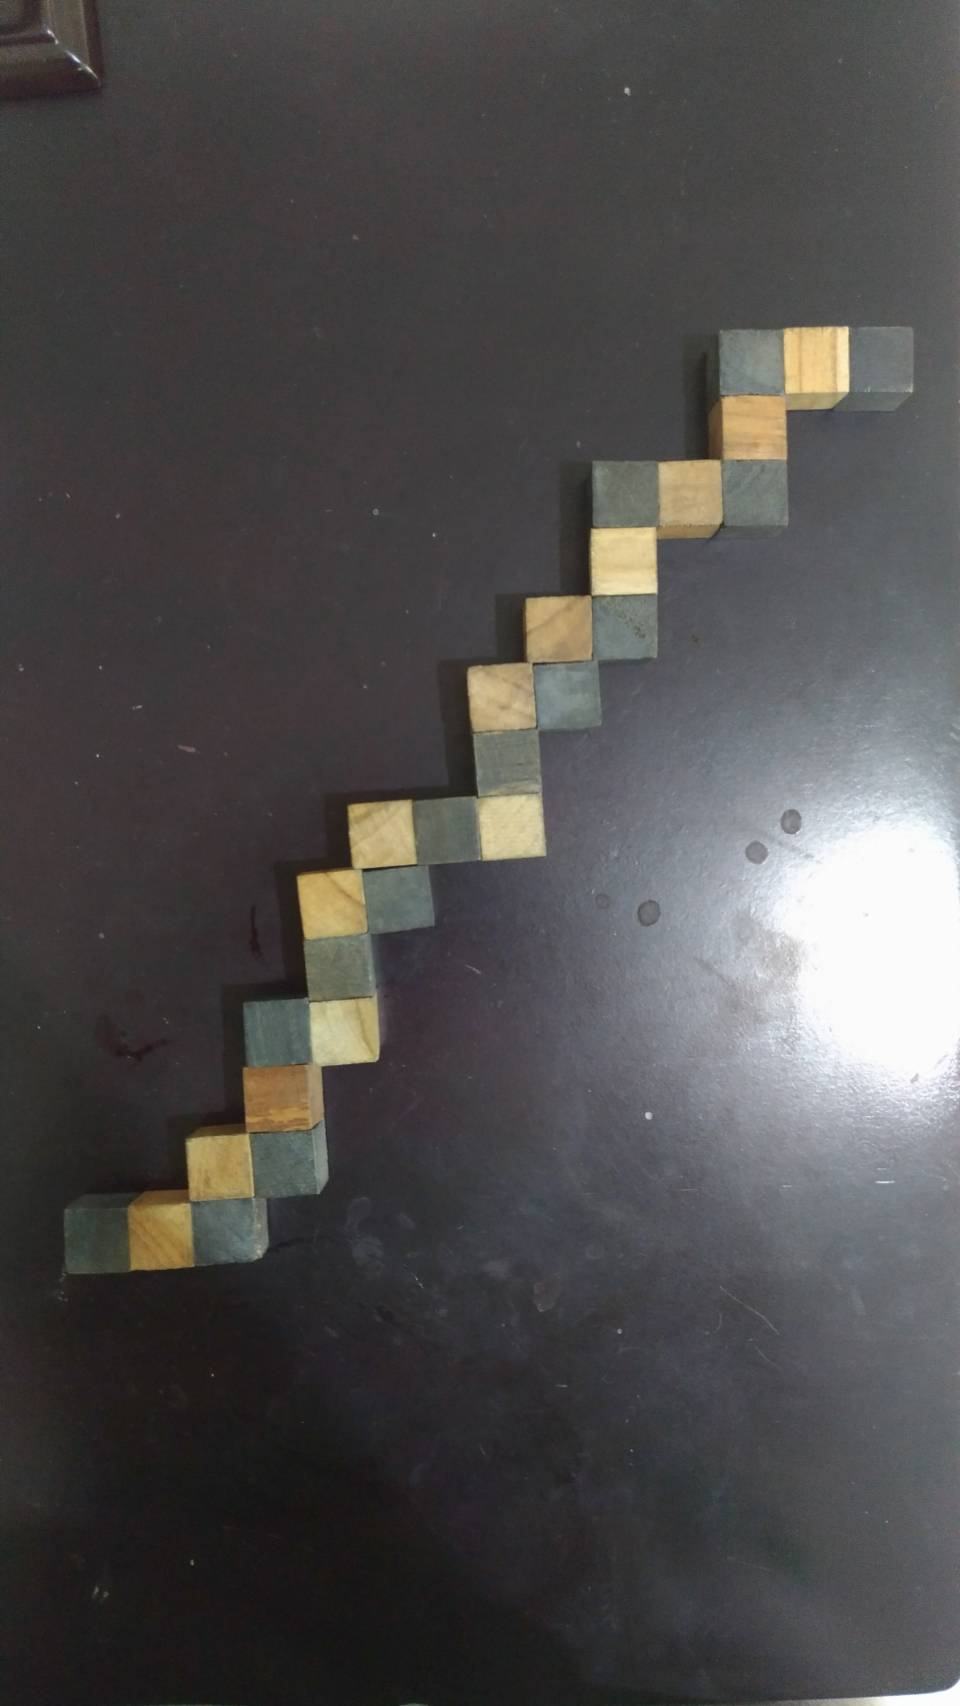
\includegraphics[width=0.4\linewidth]{sample-input.jpg}
\end{figure}

\par\noindent Ini adalah rangkaian standar yang dijual di pasaran dan dapat dibentuk menjadi kubus besar.

\subsection*{Batasan}

\begin{itemize}
	\item $2 \leq A_i \leq 3$
	\item $\sum_{i=1}^{N} A_i = 27 + N - 1$
\end{itemize}

\end{document}
